\chapter{TINJAUAN PUSTAKA}
		\section{\textit{Publish/subscribe}}
			\textit{Publish/subscribe} muncul sebahai paradigma komunikasi yang populer untuk sistem terdistribusi dalam skala yang besar. dalam \textit{publish/subscribe} \textit{consumer} akan berlangganan ke suatu \textit{event} yang diinginkan. terlepas dari kegiatan \textit{consumer}, ada \textit{event producer} yang akan menerbitkan suatu \textit{event}. jika event yang diterbitkan oleh produser cocok dengan \textit{event} yang dilanggani oleh \textit{consumer}, \textit{event} tersebut akan dikirim kepada \textit{consumer} secara \textit{asynchronus}. Interaksi ini difasilitasi oleh \textit{middleware publish/subscribe}. \textit{middleware publish/subscribe} dapat dipusatkan menjadi sebuah \textit{node} tunggal yang berperan sebagai \textit{broker} dari sebuah \textit{event} atau dipisahkan menjadi kumpulan beberapa \textit{node} \textit{broker} dari sebuah \textit{event}. 
			
			pada dasarnya, \textit{publish/subscribe} dibagi dari dua jenis yaitu: \textit{topic-based} dan \textit{content-based}. Pada \textit{topic-based publish-subscribe}, \textit{event} diterbitkan melalui sebuah topik dan \textit{consumer event} akan berlangganan topik tersebut untuk mendapatkan data dari suatu \textit{event}. berlangganan pada kasus \textit{topic-based} tidak didukung pemilahan data dari suatu \textit{event}. contohnya, \textit{consumer} akan menerima semua data dari suatu \textit{event} yang diterbikan pada suatu topik. pada \textit{content-based publish-subscribe}, berlangganan pada kasus ini didukung oleh fitur pemilahan yang diterapkan pada suatu \textit{event} yang diterbitkan. data yang dipilah oleh \textit{consumer} pada suatu \textit{event} yang berlangganan akan dikirimkan ke \textit{consumer}. \cite{noauthor_what_2016}
			
		\section{\textit{Websocket}}
          	Websocket adalah protokol berbasis TCP yang menyediakan channel komunikasi full-duplex antara server dan client melalui koneksi TCP tunggal. dibandingkan dengan skema komunikasi web real-time tradisional, protokol websocket menghemat banyak sumber daya bandwidth pada jaringan, sumber daya server, dan performa real-time yang sangat jauh lebih baik dibanding websocket tradisional. Websocket adalah protocol berbasis TCP yang independen. Websocket hanya berhubungan dengan HTTP yang memiliki handshake yang diterjemahkan oleh HTTP server sebagai pengembangan dari sebuah request. Websocket terdiri dari dua bagian yaitu: handshake dan data transfer.
           		
           	Untuk membuat koneksi Websocket, client harus mengirimkan request HTTP kepada server. setelah itu protokol akan diupgrade menjadi protokol Websocket. setelah itu server akan mengenali tipe request berdasarkan header pada HTTP. Protokol akan diupgrade menjadi Websocket apalbila diminta oleh Websocket, dan kedua kubu (client dan server) akan memulai komunikasi full-duplex, yang berarti client dan server dapat bertukar data kapanpun sampai salah satu dari client atau server menutup koneksi tersebut. Model komunikasi Websocket dapat dilihat pada gambar \ref{websocketmodel}
           		
           	Websocket memiliki kemampuan yang lebih baik dalam berkomunikasi dibandingkan dengan skema komunikasi tradisional, dimana komunikasi terjadi secara realtime. sekali koneksi sudah berhasil dibuat, server dan client melakukan aliran data dua arah, dimana aktivitas tersebut meningkatkan mempuan server untuk mengirim data. Bandingkan dengan protokol HTTP, dimana informasi yang dikirimkan lebih ringkas dan mengurangi transmisi dari data yang redundan. Dengan skala user yang besar dan kebutuhan komunikasi realtime yang tinggi, menurunkan beban pada jaringan akan menjadi keuntungan dibanding komunikasi realtime secara tradisional.
           	\begin{figure}[H]
           		\centering
           		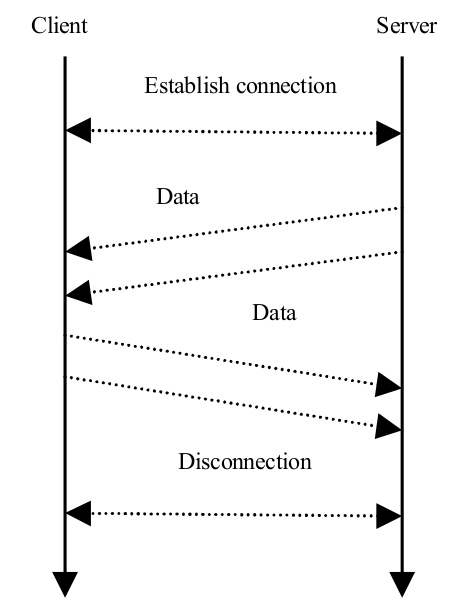
\includegraphics[height=10cm]{Images/C-2/websocket.png}
           		\caption{Model Komunikasi \textit{Websocket}}
           		\label{websocketmodel}
           	\end{figure}
           	\cite{boettiger_introduction_2015}.
		\section{\textit{SNMP}}